\section{Motivation}
{Die Ausgaben für das Internet der Dinge (IoT) wird weltweit, laut Statista, bis zum Jahr 2022 auf 1000 Milliarden US-Dollar steigen. Im Vergleich zum Jahr 2019 bedeutet dies, eine Steigerung von über 40\%.}\cite{STATISTA01:IOT} Bei einem solch starken Trend in der Informatik-Branche sollten sowohl Studenten, als auch Professoren dessen Grundlagen kennen.
Deshalb ist im Rahmen des Faches Softwarearchitektur an der technischen Hochschule Rosenheim diese Ausarbeitung geschrieben worden. Das Ziel ist es OpenHAB, ein Heimautomatisierungs-Tool, aus praktischer und technischer Sicht zu untersuchen. Außerdem wird dabei auf die Aspekte Markttauglichkeit und Benutzbarkeit in der Praxis eingegangen.

\section{Was ist OpenHAB?}
\label{s:what-is-openhab}
OpenHAB ist eine technologie-unabhängige Open-Source-Automatisierungssoftware für Smart-Homes.
Das Projekt wurde von Kai Kreuzer 2010 erstmals initiiert und wird mittlerweile durch die Community weiterentwickelt. Die Software ist hauptsächlich in Java und der Auszeichnungssprache XML geschrieben. Seit dem 16. Dezember 2019 ist die Version 2.5 erhältlich.\\
\\
Auf der offiziellen Website von OpenHAB \url{https://www.openhab.org/} sind drei klare Hauptziele definiert, die diese Software erreichen soll. Dabei ist ein Ziel die Plattformunabhängigkeit. Somit kann OpenHAB sowohl auf Linux, MacOS oder Windows betrieben werden. Auch das Hosten mit Docker oder einem Raspberry Pi wird unterstützt.\\
Weiterhin soll es durch die Plugin-Architektur möglich sein, fast jedes Gerät zu integrieren.
Es werden über 200 Technologien und mehrere tausende verschiedene Geräte unterstützt.\\
Das dritte Ziel weißt auf die vielen verschiedenen Automatisierungsmöglichkeiten hin, die OpenHAB zu bieten hat. Dabei werden Auslöser (in englisch: Trigger), Aktionen, Skripte und auch Voice-Kontrolle genannt.

\section{Bewertung OpenHAB}
In diesem Kapitel wird das open-source Projekt OpenHAB untersucht und bewertet. Es befindet sich auf Github unter \url{https://github.com/openhab/openhab-core}. Die hierfür verwendeten Kriterien sind orientiert an der QAware Open Source Quick-Check Liste.
Diese beinhaltet:
\begin{longtable}{| p{3cm} | p{12cm}|}
	\hline
	\textbf{Kriterium} & \textbf{Beschreibung} \\
	\hline \hline
	\centering Projekt Aktivität & Gibt es?
	\begin{itemize}
		\item Mindestens 1 Release im letzten Jahr
		\item Mindestens 3 aktive Contributer
		\item Stetige Commit-Aktivität von mindestens 1x pro Monat
	\end{itemize}\\
	\hline
	\centering Reifegrad & Existiert eine stabile Version > 1.0?  \\
	\hline
	\centering Lizenz & Für welche Zwecke kann das Projekt genutzt werden? \\
	\hline
	\centering Support & Existiert Issue-Tracking und ein Antwortzeit auf Tickets unter 24h? \\
	\hline
	\centering Dokumentation & Existiert?
	\begin{itemize}
		\item Api-Dokumentation
		\item Getting Started Tutorial
		\item Aktuelle Dokumentation
	\end{itemize} \\
	\hline
	\caption{OpenHAB Projektbewertungskriterien}
	\label{table:openhab-judgement-criteria}
\end{longtable}

Der Online-Dienst \textbf{Open Hub}, ehemals \textbf{Ohloh} genannt, katalogisiert opensource Softwareprojekte. Dabei werden Daten wie Projektname, Beschreibung und Sourcecode erfasst. Basierend auf diesen Daten erstellt Open Hub eine Statistik, die es ermöglicht, Codeanalyse, Projektmitarbeiter, Aktivitäten und eine Übersicht zu erhalten. Dabei werden auch viele weitere open source Projekte miteinander verglichen um aussagekräftige Statistiken und Aussagen treffen zu können.\\
\\
{In der Auswertung über OpenHAB steht beispielsweise, dass im letzten Jahr 343 Entwickler aktiv an dem Projekt mitgearbeitet haben. Somit ist OpenHAB unter den top 2\% der größten Projektteams auf Open Hub.\\
Des Weiteren ist ein stetiger Anstieg von Interesse erkennbar. Dies wird durch den Vergleich von Codebeiträgen des aktuellen Jahrs und des Vorjahres begründet.\\
Insgesamt haben über 1140 Entwickler bereits mehr als 20000 Beiträgen in Form von Programmcode zum Projekt beigetragen. Der Umfang des zu 98\% in Java geschriebenen Codes beträgt mehr als 1.5 Millionen Zeilen. Davon wurden circa 31\% dokumentiert. Dies entspricht dem durchschnittliche Wert aller Java open-source Projekte, welche auf Open Hub registriert sind.}\cite{OPENHUB01:OH} Die hierbei angegeben Werte beziehen sich auf alle Projekte und Subprojekte von OpenHAB. Eine Übersicht hierfür ist unter \url{https://github.com/openhab} zu finden.\\
\\
Wie bereits im Kapitel \ref{s:what-is-openhab} erwähnt, ist OpenHAB aktuell in der Version 2.5 erhältlich. Daraus lässt sich auf einen stabilen Codestand schließen.\\
Des Weiteren ist das Projekt unter einer EPL-2.0 Lizenz veröffentlicht. Dies erlaubt sowohl die private als auch kommerzielle Nutzung. Hinzu kommt die Möglichkeit für Modifizierung und Weiterverbreitung.\cite{LICENSE01:EC}
\\
\\
Des Weiteren wird die Qualität des Supports evaluiert. Hierfür stellt Github einen Issue-Tracker zur Verfügung. Beim Teilprojekt openhab-core wurden darüber über 1250 Issues verfasst, wovon bei circa 90\% bereits die Bearbeitung abgeschlossen ist.\cite{GITHUB01:OS} Dies lässt auf eine aktive Nutzung des Issue-Trackers schließen und bietet somit eine hilfreiche Support-Möglichkeit. Hierfür ist vor allem das Label \textbf{Bug} von Bedeutung. Eine Stichprobenartige Untersuchung von Issues dieses Types hat eine durchschnittliche Antwortzeit in unter 24h ergeben. Dies wurde anhand des ersten Kommentars gemessen. Zudem wurden bereits circa 83\% der insgesamt 68 dokumentierten Bugs gelöst.
\\
\\
Abschließend wird der Zustand der Dokumentation untersucht.
Das Getting-started Tutorial ist ausführlich und aktuell. Die darüber hinausgehende Basisdokumentation ist vollständig. Nur in Spezialfällen, wie beispielsweise der Implementierung von Services, ist die Dokumentation lückenhaft.\cite{OPENHAB01:OH}

\subsection{Fazit der Bewertung}
\begin{longtable}{| p{3cm} | p{10cm}| c |}
	\hline
	\textbf{Kriterium} & \textbf{Beschreibung} & \textbf{Erfüllt?} \\
	\hline \hline
	\centering Projekt Aktivität & Gibt es?
	\begin{itemize}
		\item Mindestens 1 Release im letzten Jahr
		\item Mindestens 3 aktive Contributer
		\item Stetige Commit-Aktivität von mindestens 1x pro Monat
	\end{itemize} & \checkmark \\
	\hline
	\centering Reifegrad & Existiert eine stabile Version > 1.0? & \checkmark \\
	\hline
	\centering Lizenz & Für welche Zwecke kann das Projekt genutzt werden? & \checkmark \\
	\hline
	\centering Support & Existiert Issue-Tracking und ein Antwortzeit auf Tickets unter 24h? & \checkmark \\
	\hline
	\centering Dokumentation & Existiert?
	\begin{itemize}
		\item Api-Dokumentation
		\item Getting Started Tutorial
		\item Aktuelle Dokumentation
	\end{itemize} & X/\checkmark \\
	\hline
	\caption{OpenHAB Projektbewertungskriterien Ergebnis}
	\label{table:openhab-judgement-criteria-result}
\end{longtable}

\subsection{Weiterführende Bewertungen}
OpenHAB wurde bereits in der Bachelorarbeit von Pirmin Gersbacher vom Jahr 2017/2018 anhand von Usecases untersucht und verglichen. Dabei kam er zu folgender Ergebnis.

\begin{minipage}{\textwidth}
	\centering
	\captionsetup{type=figure}
	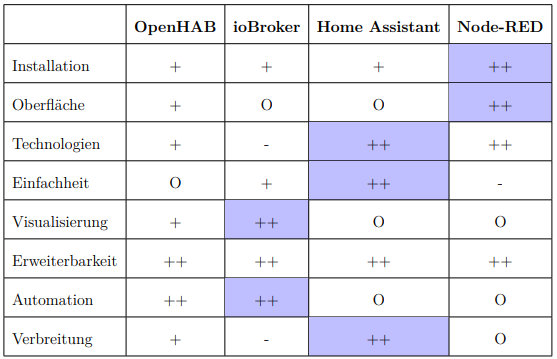
\includegraphics[width=0.8\textwidth]{\figdir/comparison-openhab.PNG}
	\caption{Vergleich OpenHAB und anderen Heimautomatisierungstools von 2017/2018 \label{fig:comparison-openhab}}
\end{minipage}

In der Tabelle \ref{fig:comparison-openhab} sind die unterschiedlichen Gebiete der Untersuchung auf der linken Seite zu finden. In der horizontalen sind die einzelnen Heimautomatisierungs-Tools aufgelistet. In der jeweiligen Zelle, basierend auf Reihe und Spalte, sind die Bewertungen festgehalten. Dabei zeigt ein blau markiertes Feld, welches das beste Tool für ein Gebiet ist.\\
OpenHAB sticht dabei nicht sonderlich heraus. Allerdings ist es in keinem der aufgelisteten Kategorien negativ bewertet.\\
Der Autor schreibt in seiner Bachelorarbeit, dass er persönlich auf OpenHAB setzen würde. Dies liegt einerseits daran, dass die Entwickler von OpenHAB stark an Vereinfachung von komplizierteren Komponenten arbeitet. Andererseits sollen aber auch komplexere Automationen, durch die Nähe von Framework und Java, möglich sein.\cite{BA01:OPH}
\\
\\
Dadurch, dass die Bachelorarbeit von P. Gersbacher vor über einem Jahr veröffentlicht wurde, stellt diese nicht mehr aktuellen Stand dar. Seitdem wurde die neuere Version 2.5 entwickelt. Diese beinhaltet einige fundamentale Veränderungen. Dabei sind Anpassungen, um eine leichtere Nutzung sicherzustellen. Auf diese Weise können sowohl OpenHAB-Entwickler, als auch Entwickler, die OpenHAB als Basis verwenden, deutlich einfacher programmieren, sagt Kai Kreuzer in seinem Online Blog Post über das OpenHAB 2.5 Release.\cite{OPENHAB02:OH}\\
In dieser Arbeit wird auf die speziellen Änderungen der Version 2.5 eingegangen. Dabei werden die Ergebnisse von P. Gersbacher als zusätzliche Quelle genutzt.


\section{openHAB aus technischer Sicht}
In diesem Kapitel werden die grundlegenden Komponenten, welche openHAB verwendet, dargestellt. Des Weiteren wird auf die  Beziehung der Komponenten untereinander eingegangen. 
Es wird ein Kern Aspekt von openHAB vorgestellt. openHAB bietet in der Regel nicht den "einen Weg". Es bietet mehrere Wege ein Ziel zu erreichen, je nach Vorlieben des Nutzers. So ist es z.B. möglich ein Gerät über die Web-Oberfläche als auch über geschriebenen Code zu integrieren. Das gleiche ist auch bei Rules zu sehen, welche entweder über ein Add-on in der Web-Oberfläche definiert werden können, oder über Code. Dieses Konzept ist ein Grundgedanken, welcher von openHAB verfolgt wird, welcher allerdings zu Verwirrung führen kann, da bei anfänglichen Umgang mit openHAB nicht unbedingt klar ist, wie man sein gewünschtes Ziel erreichen kann.
In Tabelle \ref{table:openhub-components} sind einige der Grundlegenden Komponenten aus openHAB zur schnellen Übersicht aufgeführt. Detailliert werden diese in den Entsprechenden Unterkapiteln beschrieben.

\begin{longtable}{| p{4cm} | p{11cm}|}
	\hline
	\textbf{Komponente} & \textbf{Beschreibung} \\
	\hline \hline
	\centering Add-ons & Erweiterungen, welche die Funktionalitäten von openHAB erhöhen. \\
	\hline
	\centering Bindings & openHAB-Komponenten, welche die Schnittstelle zu fremd Systemen darstellt.  \\
	\hline
	\centering Things & Repräsentation von physischen Geräten/Services in openHAB. \\
	\hline
	\centering Items & Darstellung von Eigenschaften und Ressourcen von openHAB - Thing bezogen \\
	\hline
	\centering Channels & Übertragungskanal zwischen "`Items"' und "`Things"'. \\
	\hline
	\centering Rules & Automatisierungsregeln, in Wenn-Dann-Struktur.\\
	\hline
	\centering Sitemaps & individuelle Benutzeroberfläche, welche Informationen präsentiert und Interaktionen ermöglicht.\\
	\hline
	\caption{OpenHAB Komponenten}
	\label{table:openhub-components}
\end{longtable}

\subsection{Add-ons}
openHAB setzt verwendet das Konzept von Add-ons als Teil ihrer zusammen steckbaren Architektur (pluggable architecture). Dadurch dass vordefinierte Bereiche von openHAB erweitert werden können, wird openHAB der Anforderung gerecht "alles" zu Integrieren. Das Konzept der Add-ons ermöglicht es außerdem nur Benötigte Module zu installieren bzw. zu verwenden wodurch openHAB schlank, leicht und überschaubar bleibt. Die Bereiche in denen openHAB offen ist um erweitert zu werden sind:
\begin{itemize}
	\item Bindings
	\item Automation Engine Modules
	\item Transformations / Profiles
	\item IO Services
	\item Persistence Services
	\item Audio \& Voice
\end{itemize}
Um den Rahmen dieser Arbeit nicht zu übersteigen wird nur auf Bindings detaillierter eingegangen, siehe Kapitel \ref{sec:Bindings}. Bei den nicht näher Beschriebenen Add-ons handelt es bei Automation-Engine-Modules um Bedingungen oder Aktionen, welche für Rules oder Scripte verwendet werden können. Transformations / Profiles können genutzt werden um Werte welche durch Channels übertragen werden zu tranformieren/modfizieren. IO Services sind ermöglichen es interne Schnittstellen von openHAB nach außen aufzumachen, dies geschieht z.B. bei der REST-Api, dem HomeKit für Apple oder dem Hue Emulation Service für Philips. Persistence Services können genutzt werden um den Status von Items z.B. in Datenbanken abzuspeichern und wieder Abzurufen. Und bei Audio \& Voice handelt sich um Services welche genutzt werden können um Audioquellen abzuspielen oder Stimminteraktionen mit Nutzern zu ermöglichen. 

\subsection{Bindings} \label{sec:Bindings}
Bindings sind die Komponenten, welche es ermöglicht Systeme oder Geräte mit openHAB zu integrieren. Mit einem Binding kann sowohl ein physisches Geräte wie z.B. eine LG Fernseher mit WebOS als auch eine Service z.B. Spotify angebunden werden. Die Bindings sind dabei meist soweit abstrahiert, dass nicht jedes einzelne Model bzw. Version eine eigenes Binding benötigt.
Nach der Installation eines Bindings, was über die Web-Oberfläche oder per Code passieren kann, ist openHAB in der Lage Geräte/Systeme im Netzwerk zu finden. Mittels Bindings können auch Geräte/Systeme integriert werden, welche wiederum die Steuerung für andere Geräte übernehmen z.B. Hue-Bridge oder Bluetooth. Diese Geräte/Systeme wiederum ermöglichen es i.d.R. nach dem Hinzufügen in openHAB, dass durch das Binding Kindkomponenten gefunden und ebenfalls zu openHAB hinzugefügt werden können. Dadurch ist es möglich, wie im Falle des Hue-Systems nicht nur die Hue-Bridge, sondern alle mit der Hue-Bridge verbundenen Lampen einzeln in openHAB zu integrieren und dadurch zu steuern. Dieses ansteuern von einzelnen Kindkomponenten im Falle des Hue-Systems, wäre durch ZigBee theoretisch möglich, würde aber einen sehr hohen und unnötigen Aufwand bedeuten. 
Laut openHAB gibt es aktuell über 300 Bindings welche es ermöglichen über 2000 Things anzusprechen.

\subsection{Things}
Things stellen die Repräsentation von physischen Geräten/Services innerhalb von openHAB dar. Sie bestehen neben verschiedenen Status und Konfigurationsinformationen aus Channels, welche für die Ansteuerung der Things benötigt werden und näher in Kapitel \ref{sec:channels} beschrieben werden.
Things können auf drei verschiedene Arten openHAB hinzugefügt werden. Diese sind:
\begin{itemize}
	\item per Web-Oberfläche automatisch: Nachdem das für das Thing benötigte Binding installiert wurde, erscheint das Thing in der Inbox, siehe Abbildung \ref{fig:thing-add-paper-ui}. Von dieser Inbox aus, kann das Thing mit wenigen Klicks openHAB hinzugefügt werden. Durch diese Methode werden alle nötigen Einstellungen für das Thing automatisch getroffen. Diese können nachträglich bearbeitet werden z.B. die Bezeichnung. 
\end{itemize}
{\centering
\captionsetup{type=figure}
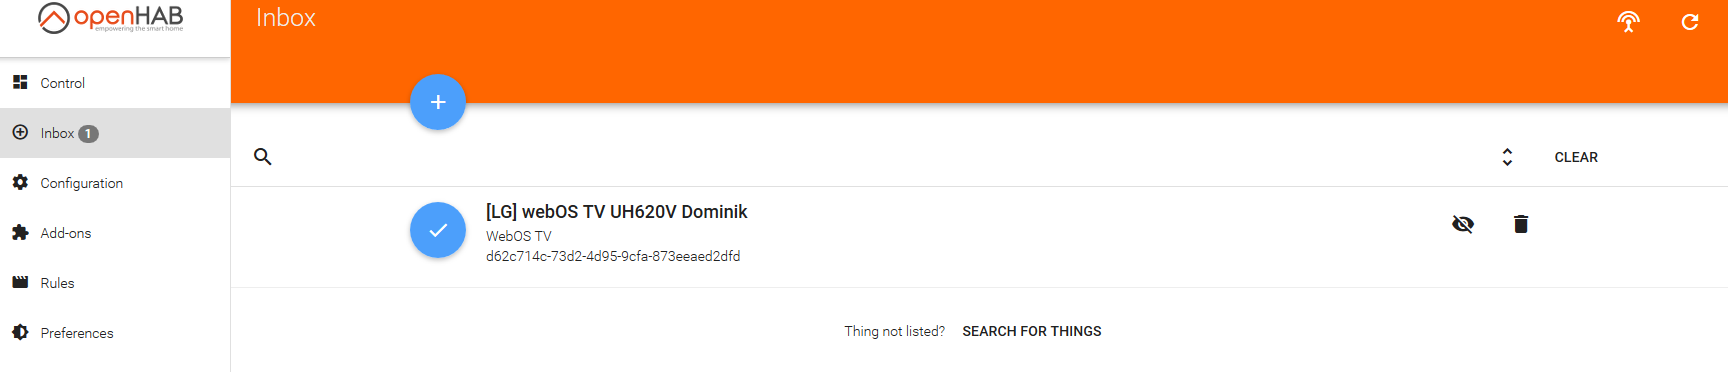
\includegraphics[width=1\textwidth]{\figdir/thing_add.PNG}
\caption{Thing per Web-Oberfläche \label{fig:thing-add-paper-ui}}
}	
\begin{itemize}	
	\item per Web-Oberfläche Manuell: Das manuelle Hinzufügen von Things ermöglicht volle Einstellungsfreiheit für Things. Dazu zählen ID, Bezeichnung, IP-Adresse und Konfigurationsparameter. Dies ist in Abbildung \ref{fig:thing-add-paper-ui-manuel} zu sehen. Diese Einstellungsfreiheit setzt allerdings auch voraus, dass der Nutzer weiß, welche Informationen er in welches Feld eintragen will/muss. Genau wie bei dem automatischen erkennen, können die Einstellungen noch nachträglich geändert werden. 
\end{itemize}
{
	\centering
	\captionsetup{type=figure}
	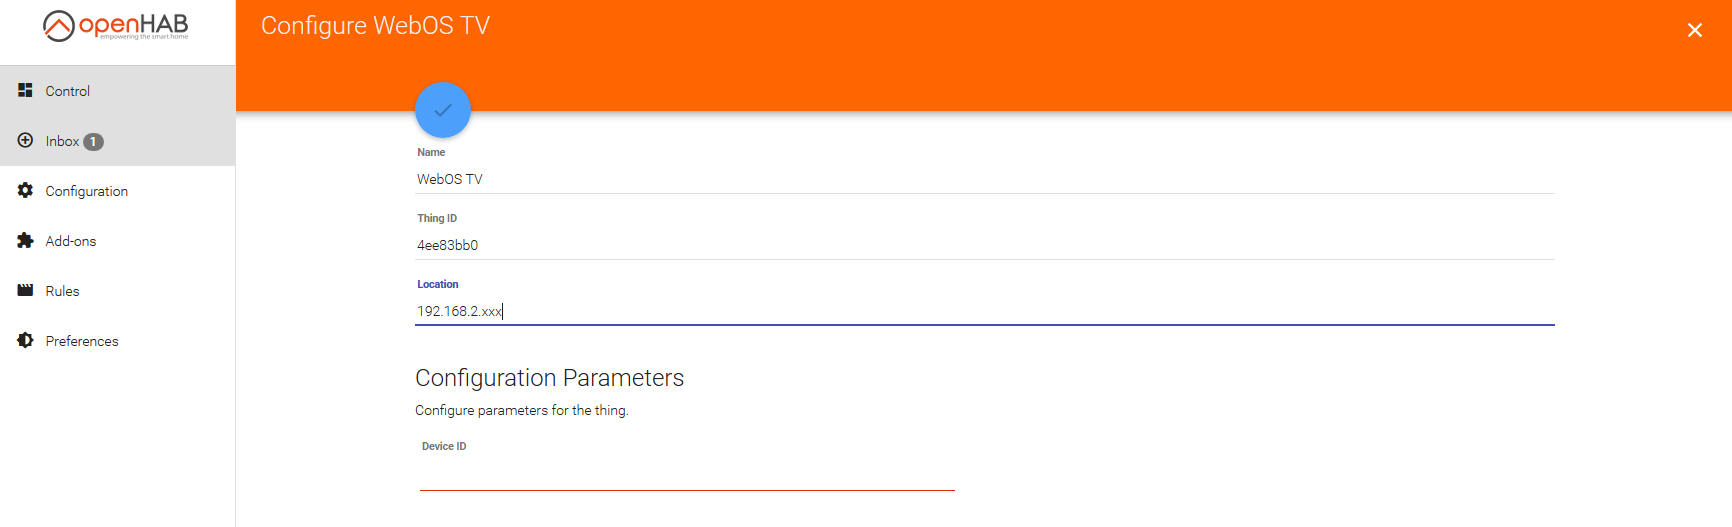
\includegraphics[width=1\textwidth]{\figdir/thing_add_manuel.PNG}
	\caption{Thing per Web-Oberfläche Manuell \label{fig:thing-add-paper-ui-manuel}}
}
\begin{itemize}	
	\item per Code. Ermöglicht und benötigte komplette manuelle Eingabe aller nötigen Informationen im Dateiordner  \textit{openHAB-config/things/}. Diese sind wie im einfachen Beispiel Abbildung \ref{fig:thing-add-code} Binding-Pfad, IP-Adresse, und ID. Um dies zu vereinfachen sind in der Dokumentation Beispiele für die verschiedenen Bindings mit zugehörigen Things zu finden.
\end{itemize}
{
	\centering
	\captionsetup{type=figure}
	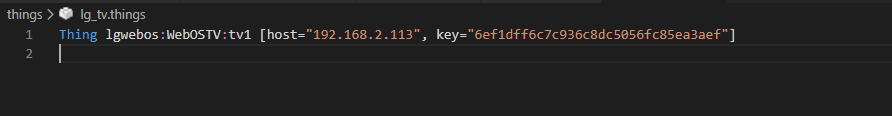
\includegraphics[width=1\textwidth]{\figdir/thing_add_code.PNG}
	\caption{Thing per Code \label{fig:thing-add-code}}
}

\subsection{Channels} \label{sec:channels}
Channels sind Kommunikationswege welche von Things angeboten werden und diese mit Items verbinden. Mit Hilfe der Channels werden Aktionen, welche Things auszuführen haben Parameter übergeben. So bietet der verwendete LG Fernseher wie in Abbildung \ref{fig:channel-list} zu sehen eine Liste von Channels an, welche Daten für Aktionen übertragen um diese Auszuführen. Das heißt, dass Channels sowohl die Kommunikationswege mit zugehörigen Parameter repräsentieren, als auch Aktionen, welche Things ausführen können. Da ein gewünschte Aktion eines Things ohne den passenden Channel diese Aktion nicht ausführen kann.

{
	\centering
	\captionsetup{type=figure}
	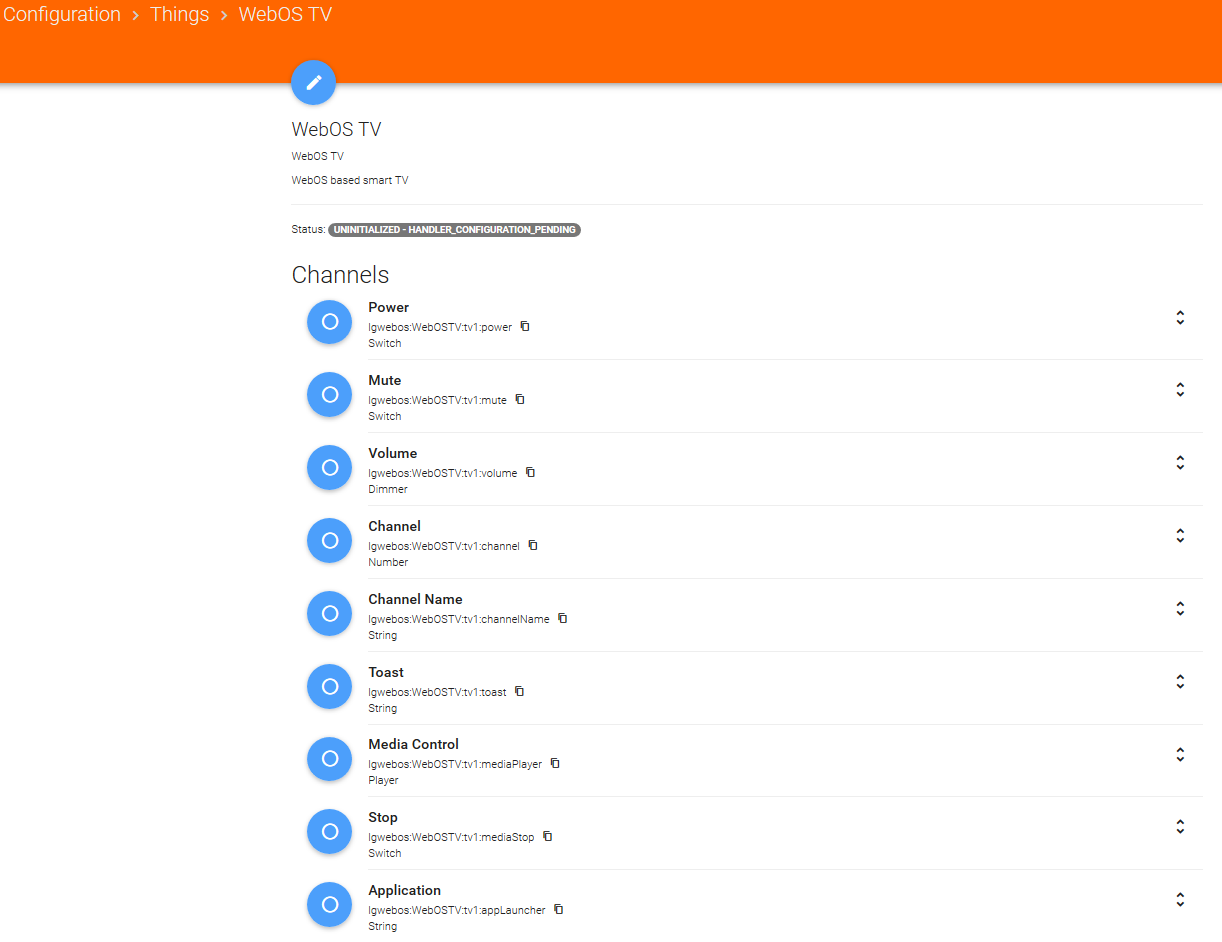
\includegraphics[width=1\textwidth]{\figdir/channel-list.PNG}
	\caption{Channel Liste\label{fig:channel-list}}
}

\subsection{Items}
Der Begriff Item oder zu deutsch Ding, kann missverständlich aufgefasst werden. Bei einem Item handelt es sich um alle Informationen, welche es um eine Aktion gibt. So hat ein Item u.a. Bezeichnung, Kategorie, Typ, Status als auch Konfigurationen z.B. dass nur Werte von 0 - 50 übertragen werden. Diese Informationen werden benötigt um Gruppierungen zu ermöglichen, den Status eines Gerätes abzufragen z.B. Lautstärke eines Fernsehers und auch mit einem Thing zu kommunizieren bzw. Aktionen auszuführen. Der Typ eines Items gibt an, welche Basistypen von dem Item akzeptiert/konsumiert werden können. Solche Basistypen können einfache aus der Programmierung bekannte Typen wie String, Number, DateTime usw. sein, als auch komplexere openHAB spezifische Typen wie Location, Player oder Switch. Eine komlpette Auflistung ist unter \url{https://www.openhab.org/docs/configuration/items.html#type} zu finden.

Items sind essentielle um Aktionen auf der Web-Oberfläche dazustellen. So können diese in Gruppen oder Einzeln dargestellt werden um als Statusanzeige und/oder als manuelle Steuerung des Smart Home zu agieren. Für diese Steuerung ist anzumerken, dass jedem Item nur ein Channel zugeordnet werden kann, aber jedem Channel mehrere Items. Die Kardinalität ist somit Item 1 -> n Channel. 

Items können wie bei openHAB üblich ebenfalls über die Web-Oberfläche als auch im Code erzeugt werden. Da dieses Prinzip schon hinreichend erklärt wurde, wird mit Ausnahme der automatischen Namensgebung nicht näher darauf eingegangen. Diese Namensgebung ist in erster Linie frei, jedoch vergibt openHAB über die Web-Oberfläche als Item-Name eine Kombination aus Thing- und Channel-Namen wodurch sehr gut ersichtlich wird, wofür ein Item genutz werde kann z.B. \textit{LGWebOSTVUH620V\_VolumeTV} oder \textit{HueWhiteLamp1\_Brightness}.

\subsection{Rules}
Automatisierung in openHAB findet durch Rules/Scripte statt. Diese Rules werden aktuell standardmäßig durch Programmieren erzeugt. Um Rules zu erzeugen, wird eine einfache WENN-DANN-Struktur verwendet. Diese Regeln können auf verschiedene Bedingungen "lauschen". So können Bedingungen (WENN) von Items, Member of (Gruppierungen), Time, System oder Things stammen. Genauer kann die Bedingung durch eine verschiedene Formen eingeschränkt werden wie z.B. received command [<command>],  received update [<state>] oder changed [from <state>] [to <state>] usw.
Wenn diese Bedingung erfüllt ist, wird im DANN-Pfad die Reaktion definiert. So können Item oder Ganze Gruppen von Items angesprochen werden. Hierbei wird dadurch ein/jedes Item Informationen an Channels weitergeben, welche eine Aktion bei dem dazu gehörigen Thing auslöst.
Wie im Codebeispiel \ref{lst:sample-rule} zu sehen, gibt es die Möglichkeit innerhalb des DANN-Blocks weitere Strukturelemente einzufügen um aus mehreren Rules eine zu machen.

Alternativ zur Programmierung ist es mit einem experimentelles Add-on möglich, über die Web-Oberfläche Rules zu definiert. Allerdings ist hier anzumerken, dass komplexere Regeln schwierig bis gar nicht zu erzeugen sind. Dies liegt daran, dass die Eingabemöglichkeiten beschränkt sind und durch das Konvertieren in das JSON-Format z.B. Sonderzeichen wie  \textit{>,<,=,!} nicht funktionieren. Des Weiteren ist das einfügen von zusätzlichen Strukturelementen über das experimentelle Add-on nicht möglich.

\begin{lstlisting}[language=java,firstnumber=1,caption=Rule Beispiel,label=lst:sample-rule]
rule "React on Volume (LGWebOSTVUH620VDominik_Volume) change"
when
	Item LGWebOSTVUH620VDominik_Volume changed
then
	logDebug("React some changes on Volume", "current Value: " + LGWebOSTVUH620VDominik_Volume.state.toString)
if ( LGWebOSTVUH620VDominik_Volume.state >= 20 ) {
	HueWhiteLamp2_Brightness.sendCommand(80)
}
else {
	HueWhiteLamp2_Brightness.sendCommand(5)
}
end
\end{lstlisting}

\subsection{Sitemaps}
Sitemaps dienen als Übersicht, Gruppierung und Visualisierung des Smart-Homes. So werde durch Sitemaps räume nachbildet um Komplette beleuchtung innerhalb eines Raums ein/auszuschalten, Temperatur o.ä. im Auge zu behalten. Neben Sitemaps können auch ander Darstellung wie Panels verwendet werden. SiteMap und Dashboards dienen wie der Name schon sagt als Dashboard (Wie blöd kann ich denn das schreiben). Und als kontrolleinheit für das Smart-Home. Die Erstellung wird durch eiditoren errleichtert, welche Programmierunkundigen Code-Snippits zur Verfüfung stellt.

\subsection{Api}
OpenHAB nutzt um die Paper-UI zu nutzen eine REST-API. Diese ist offengelegt, was anderen Systemen es ermöglicht die Komplette Funktionalität, welche über die Web-Oberfläche nutzbar ist ebenfalls zu integrieren. Dies ermöglicht es unter anderem Entwicklungsumgebungen wie VS-Code, Eclipse, IntelliJ Add-Ons/Extensions zu entwickeln, welche das Prgrammieren für OpenHab vereinfacht. So bieten diese 3 Extensions welche die Rest-Api nutzen um ITEMS und Things welche im System verfügbar sind anzuzeigen, was es sehr angenehm macht Rules o.ä. zu entwickeln.
Die Rest-API ermöglicht es ebenfalls unabhänigen entwicklern openHAB funktionen zu steuern, was allerdings im Mobilen bereich irrelevant sein sollte, da es android, ios und windows apps bereits gibt


\subsection{Entwickeln für OpenHAB??} \label{sec:custom-development}


OpenHab bietet zusätzlich zur Dokumentation noch Untestützung für das Entwickeln eines Eigenen Bindings durch eine Skeletton skript, welches die Stuktur eines Bindings inklusive Beispielen und Erklärungen welche Methonde/Funktionen wie gestaltet werden müssen und was diese Tun. Siehe:
\captionsetup{type=figure}
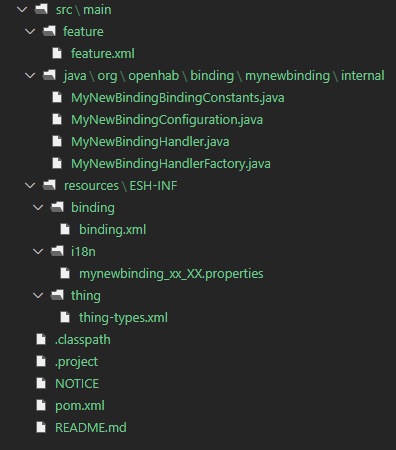
\includegraphics[width=0.5\textwidth]{\figdir/own_binding_skeletton.PNG}
\caption{Skelett für Binding \label{fig:own_binding_skeletton}}

OpenHAB liefert für das Entwickeln von Add-Ons Skelleton-Skripte, welche die von openHAB bentigte Struktur erzeugen. Für manuelles Hinzufügen von Things, Items, Rules usw. bietet openHAB bereits eine ORdnerstruktur. Diese ist so offensichtlich, dass es trivial ist zu entscheiden, wo welche Komponente hinzugefügt werde soll. Sollte dies dennoch unklar sein, wird der Nutzer noch weiter durch readme-dateien unterstützt. Siehe 

entwicklung von IO-, Persistence Services und Audio/Voice mit einem TODO beschreibt eher dürftig ist.


Sollte es allerdings keine passendes Add-on für ein gewünschtes Gerät geben, steht der erweituerng und dem entwicklen eines eigenenen Add-ons durch das Add-on System nichts im Weg. Mehr noch, durch den OpenSource gedanken, welcher openHAB vorantreibt könnte das Gesamt-System durch ein weiteres Add-on erweitert werden.
\captionsetup{type=figure}
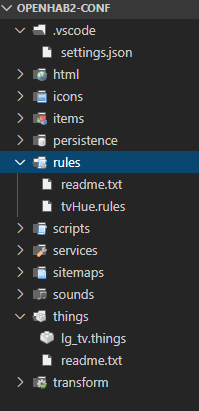
\includegraphics[width=0.25\textwidth]{\figdir/openHab-conf-folder-structure.PNG}
\caption{openHAB-conf Ordnerstruktur \label{fig:openHab-conf-folder-structure}}



ich muss mir noch überlegen, ob ich daraus ein eigenes kapitel mach, oder ob e sunter die anderen bauch.
\url{https://www.openhab.org/docs/configuration/restdocs.html}
\begin{itemize}
	\item Item ein-/ausschalten
	\item Eine List von allen Items, Sitemaps ausgeben lassen
	\item Mit einem Editor auf die ganzen Komponenten zugreifen:
	\begin{itemize}
		\item Visual Studio Code installieren
		\item Openhab Extension installieren
		\item Geteiltes Openhab Laufwerk als Ordner öffnen
		\item Openhab Extension konfigurieren
		\item Es werden auch andere Editoren unterstützt
	\end{itemize}
\end{itemize}

\section{Datenintegrität und Sicherheit}
\begin{itemize}
	 \item It is known that security breaches may have a significant economic impact on a firm, as
	 described by Goel and Shawky [18]. Data loss or theft, tampering, and unauthorized
	 operations are just some of the possible ocurrences led by the lack of proper security
	 mechanisms in place. In the case of openHAB, a smart home application, it is not quite
	 quantifiable how expensive it results to have a security breach occur at any level. The
	 consequences may go from mere user discomfort to identity theft, or worse.
	\item \url{https://www.owasp.org/index.php/OWASP_Internet_of_Things_Project}
	\item \url{https://www.google.de/url?sa=t&rct=j&q=&esrc=s&source=web&cd=7&ved=2ahUKEwjq_c-k0s7mAhXOIVAKHS4dDYgQFjAGegQICBAC&url=https%3A%2F%2Fcomserv.cs.ut.ee%2Fhome%2Ffiles%2FSoto_computer_science_2018.pdf%3Fstudy%3DATILoputoo%26reference%3DB7FBB08D43717164067F1F9DBA92B98A65913AC9&usg=AOvVaw0631sYhHX3wKxW8kPwxpzE}
	\item Weak, Guessable or Hardcoded Passwords: Easy to brute force (no captcha), unchangable credentials
	\item Masterarbeit gefunden -> Status ist veraltet -> Checken, was sich seitdem bei OpenHAB getan hat -> keine wirklich relevanten security changes alexa und google home.
	\item 2.4 hat auch nur kleine security Changes für GPS Tracker Binding
\end{itemize}
\subsection{Interne vorhandene Funktionalitäten}
\url{https://www.openhab.org/docs/installation/security.html}
\begin{itemize}
	\item Through the command line console, which is done through SSH and thus always authenticated and encrypted. You will find all details about this in the Console documentation.
	\item Through HTTP(S) over \url{https://<ip>:8443}
	\item SSL Certificates
	On the very first start, openHAB generates a personal (self-signed, 256-bit ECC) SSL certificate and stores it in the Jetty keystore (in \${USER\_DATA}etc/keystore). This process makes sure that every installation has an individual certificate, so that nobody else can falsely mimic your server. Note that on slow hardware, this certificate generation can take up to several minutes, so be patient on a first start - it is all for your own security.
	\item Security Warning: It is vitally important that you MUST NOT directly expose your openHAB instance to the Internet (e.g. by opening a port in your firewall)!
\end{itemize}
\begin{minipage}{\textwidth}
	\centering
	\captionsetup{type=figure}
	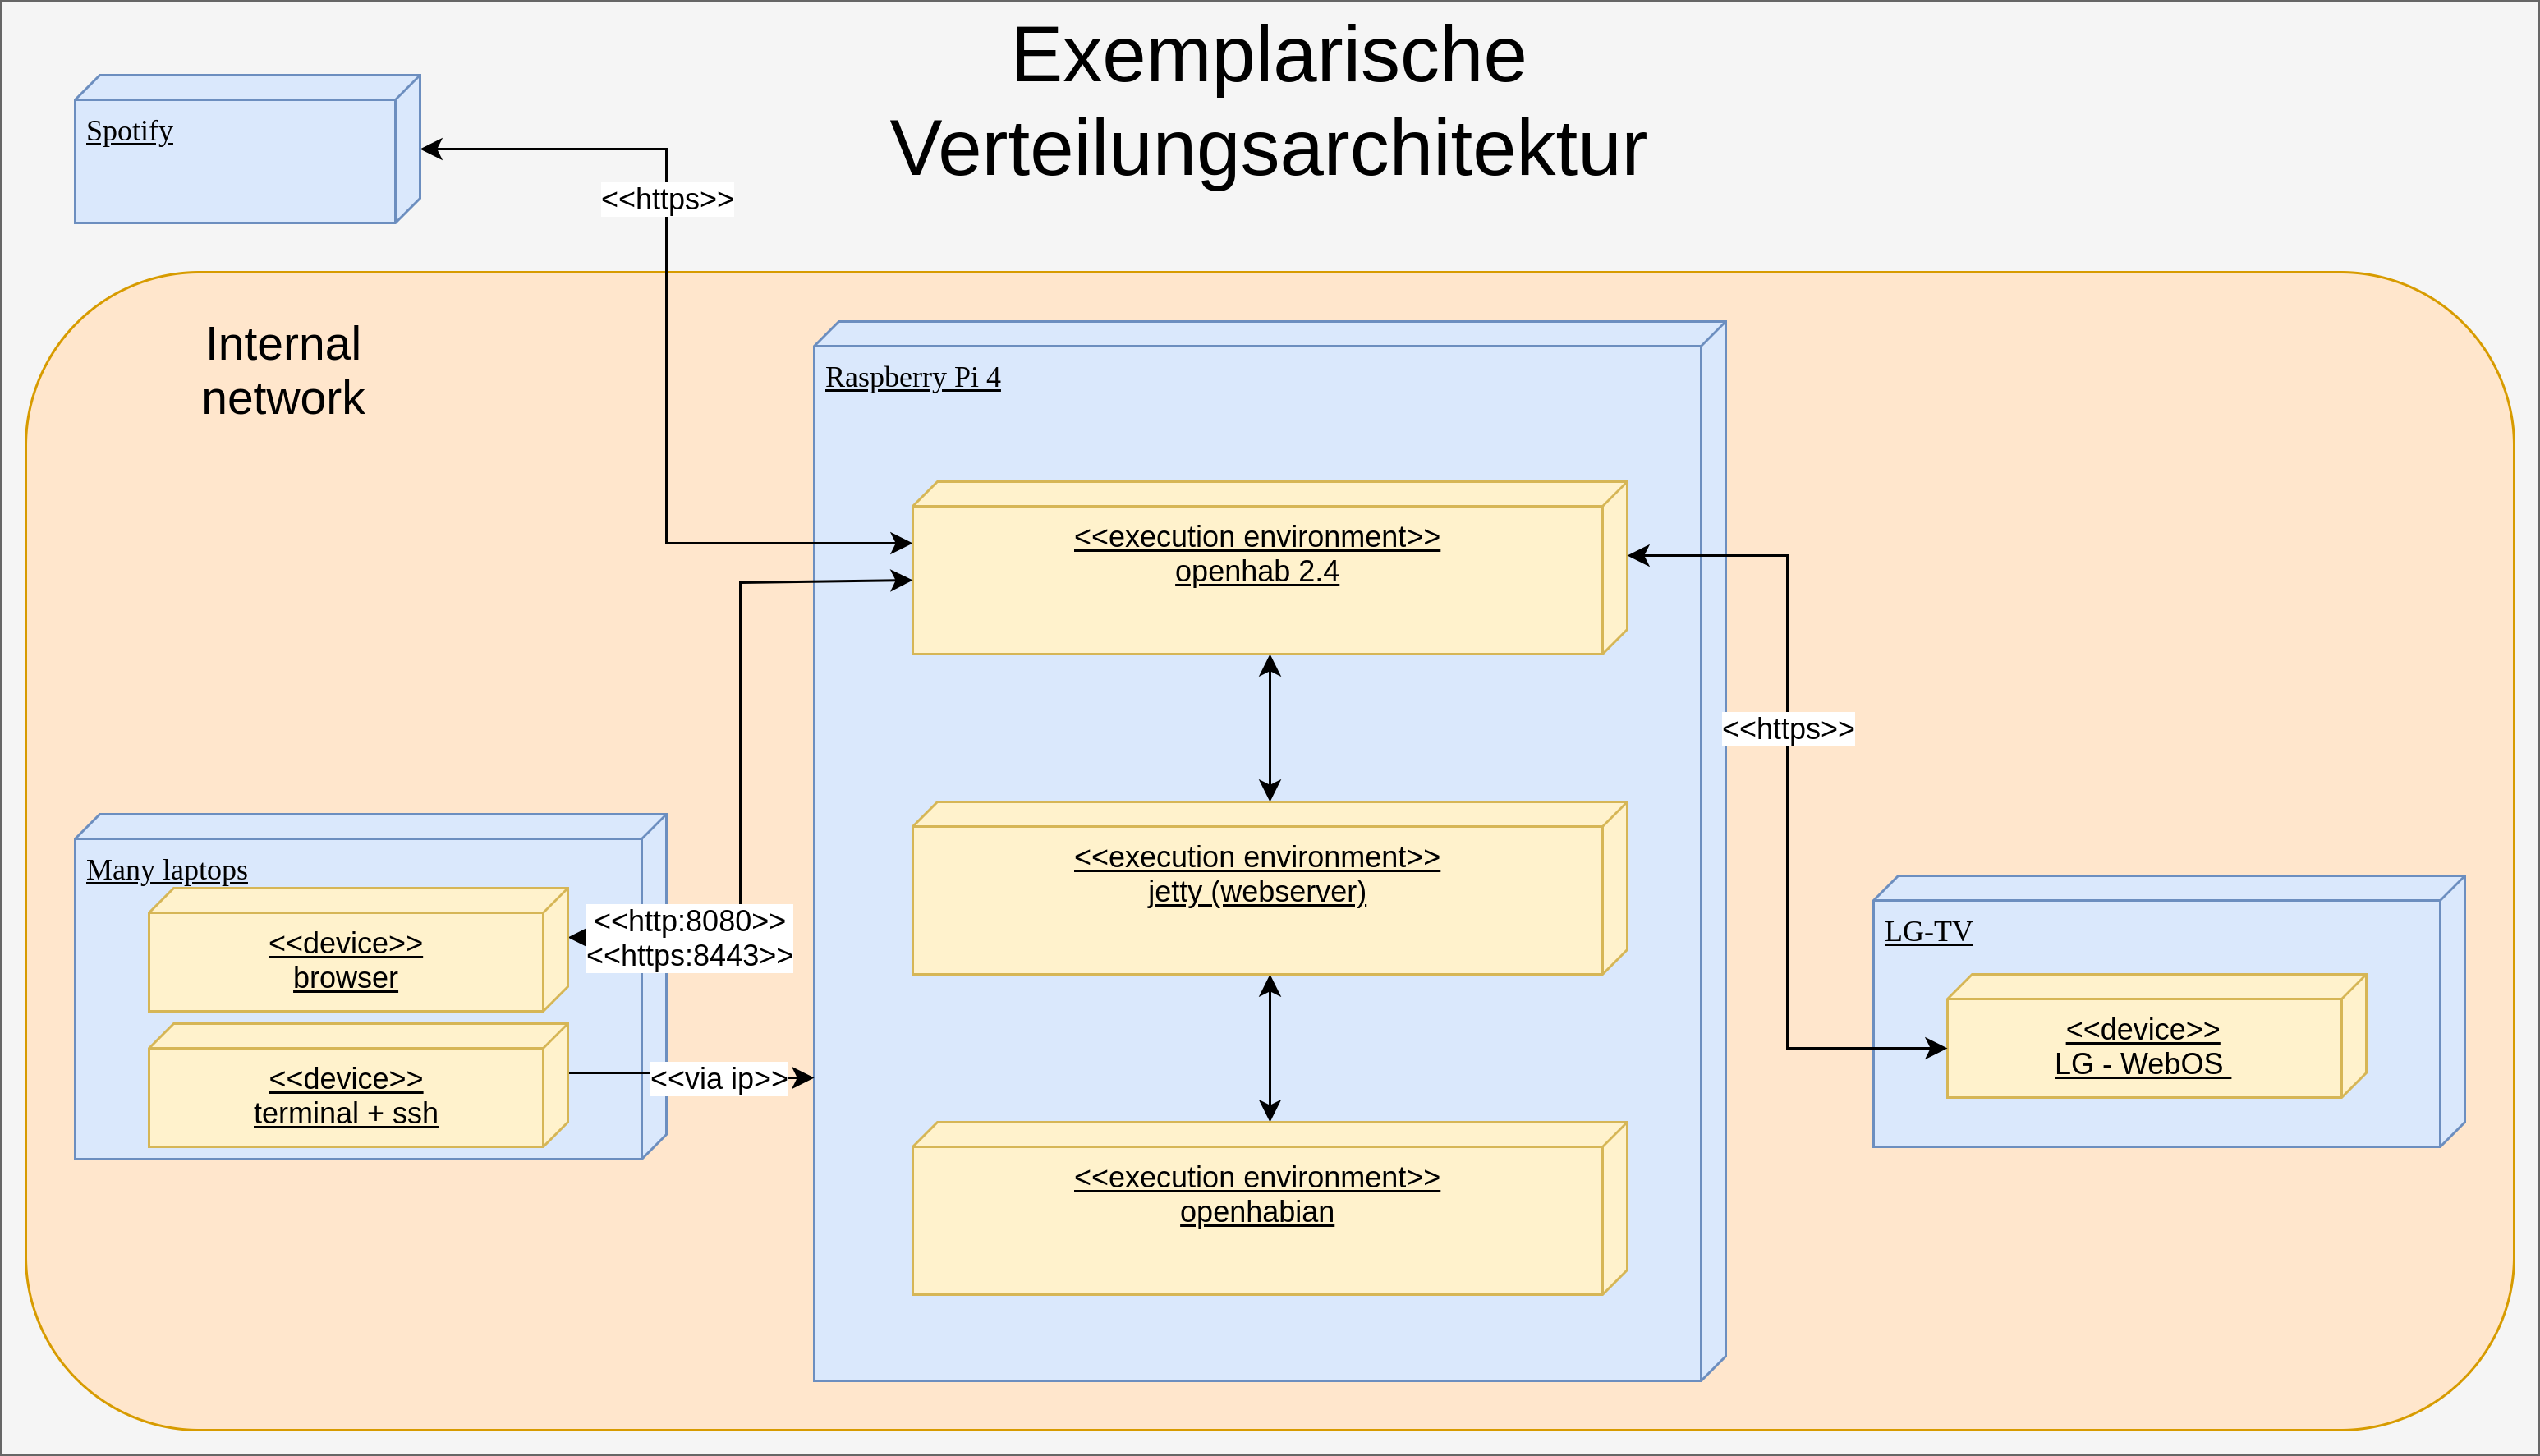
\includegraphics[width=1\textwidth]{\figdir/verteilungsarchitektur.png}
	\caption{Übersicht einer exemplarischen Anwendung von OpenHAB \label{fig:verteilungs-architektur}}
\end{minipage}
\subsection{Externe Erweiterungsmöglichkeiten}
\begin{itemize}
	\item Options for Secure Remote Access
	\begin{itemize}
		\item VPN: The most secure option is probably to create a VPN connection to your home network
		\item myopenHAB Cloud Service with a tunnel that forwards all requests to the openHAB instance
		\item Running openHAB Behind a Reverse Proxy: A reverse proxy simply directs client requests to the appropriate server. This means you can proxy connections to \url{http://mydomain_or_myip} to your openHAB runtime.
	\end{itemize}
\end{itemize}

\section{Verwendung von OpenHAB}
\subsection{Integration der Big Player}
\begin{itemize}
	\item Amazon Alexa und Echo Dot Integration möglich
	\item Changes die mit v2.5 released wurden miteinbauen in das Kapitel:
	\url{https://www.openhab.org/blog/2019-12-14-openhab-2-5-release.html}
	\begin{itemize}
		\item Alexa:
		\begin{itemize}
			\item This certified Amazon Smart Home Skill allows users to control their openHAB powered smart home with natural voice commands. Lights, locks, thermostats, AV devices, sensors and many other device types can be controlled through a user's Alexa powered device like the Echo or Dot.
			\item \url{https://www.openhab.org/docs/ecosystem/alexa/}
			\item \url{https://www.openhab.org/addons/bindings/amazonechocontrol/}
		\end{itemize} 
		\item Google Home
		\begin{itemize}
			\item Google Home Integration möglich
			\item With the Action you can voice control your openHAB items and it supports lights, plugs, switches and thermostats. The openHAB Action comes with multiple language support like English, German or French language.
			\item The openHAB Action links your openHAB setup through the myopenHAB.org cloud service to the Google Assistant platform
			\item openHAB Cloud Connector configured using myopenHAB.org . (Items DO NOT need to be exposed to and will not show up on myopenHAB.org
			, this is only needed for the IFTTT service!)
			Google account.
			Google Home or Google Home mini.
			
			\url{https://www.openhab.org/docs/ecosystem/google-assistant/}
		\end{itemize} 
	\end{itemize}
	
\end{itemize}

\subsection{Beispiel Aufbau eines OpenHAB Smart-Homes}
\begin{itemize}
	\item OpenHAB auf Raspberry Pi 3/4 installiert
	\item Welche Geräte haben wir mit OpenHAB verbunden?
	\begin{itemize}
		\item Spotify
		\begin{itemize}
			\item Lautstärkeregler
			\item Aktueller Song Display
		\end{itemize}
		\item LG Smart TV
		\begin{itemize}
			\item Lautstärkeregler
			\item An- und ausschalten
			\item One-Way-Chat
		\end{itemize}
		\item Lampen
	\end{itemize}
	\item Wie haben wir die Geräte verbunden?
	\begin{itemize}
		\item \textbf{Verschiedene Binding:}
		\item Spotify Binding
		\item LG Smart TV Binding
	\end{itemize}
	\item On the server the configuration is stored somewhere in userdata (/var/lib/openhab2 for apt-get installs).
	In an upgrade the userdata folder is preserved when using apt-get.
\end{itemize}

\begin{minipage}{\textwidth}
	\centering
	\captionsetup{type=figure}
	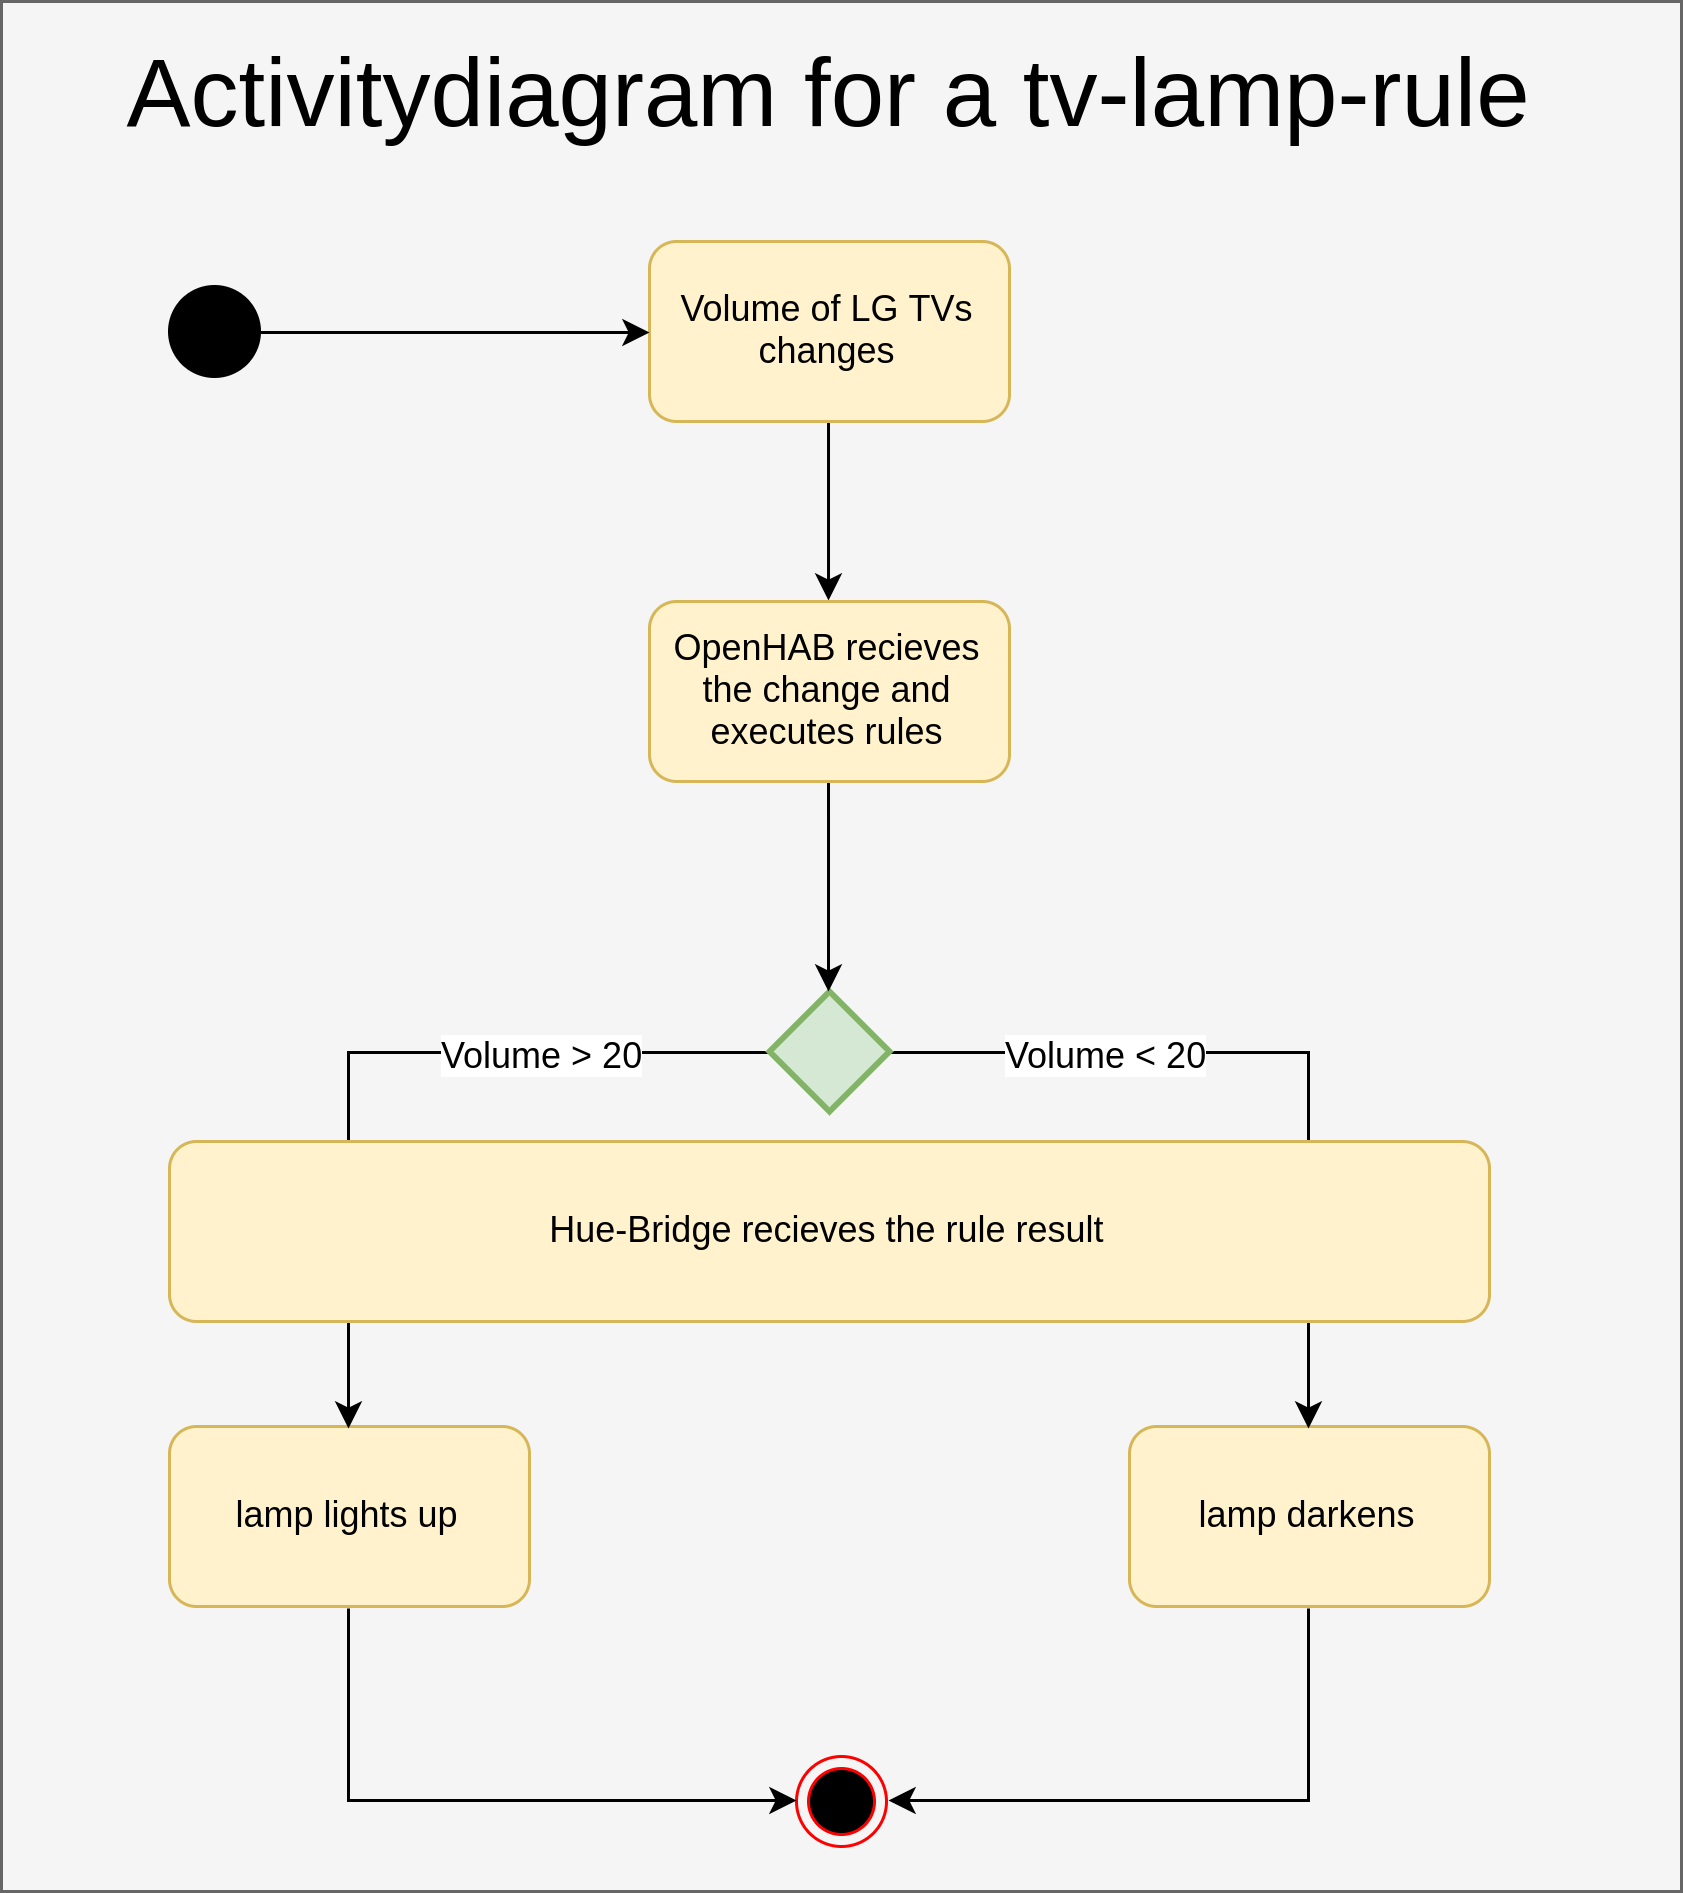
\includegraphics[width=1\textwidth]{\figdir/activitydiagram-lg-light-rule.png}
	\caption{Aktivitätsdiagram für eine Rule \label{fig:activity-diagram}}
\end{minipage}

\subsection{Umgang mit OpenHAB}
\begin{itemize}
	\item Das meiste klickt mans ich zusammen: Bindings, Rules, Channels, Items, Things
	\item Implementierung von rules scheint idiotensicher, weil:
	\begin{itemize}
		\item einfacher Syntax
		\item Abhängigkeiten managed Openhab
	\end{itemize}
	\item Bindings schreiben scheint eher schwieriger
\end{itemize}

\section{Fazit}
\subsection{Stärken}
Some of openHAB's strengths are:

Its ability to integrate a multitude of other devices and systems. openHAB includes other home automation systems, (smart) devices and other technologies into a single solution
To provide a uniform user interface and a common approach to automation rules across the entire system, regardless of the number of manufacturers and sub-systems involved
Giving you the most flexible tool available to make almost any home automation wish come true; if you can think it, odds are that you can implement it with openHAB.
\subsection{Schwächen}
\textbf{Wollen wir das hier als SWOT Analyse aufziehen?}
\begin{itemize}
	\item Integration von USB-Geräten scheint eher kompliziert. Vor allem auf Raspberry Pi
	\item Serial Binding wird nicht angezeigt
	\begin{itemize}
		\item Mikrofon an Raspberry Pi oder anderes Geräte verbinden
		\item Input des Mikrofons über OpenHAB an ein Ausgabegerät, wie zum Beispiel eine Bluetooth Box, senden und abspielen
		\item Raspberry hat da auch für große Probleme bei der Geräteerkennung gesorgt - USB gerät wurde nicht im devices Verzeichnis aufgeführt und somit konnte auch keine Verbindung mit OpenHAB aufgebaut werden
		\item OpenHAB Serial Device Binding wurde auch nicht angezeigt, um Geräte darüber zu suchen
	\end{itemize}
\end{itemize}

\section{Outlook}
Outlook
With the 2.5 release build, our development master branch has now become 3.0.0. This means that there will most likely be no openHAB 2.6 runtime in future, while there will still be 2.x updates on the add-ons, though. The focus of the core maintainers will clearly be on openHAB 3 from now on, which will bring bigger changes that have been discussed since a while: The existing UIs will be replaced by a single one, completely implemented from scratch. The "next-generation" rule engine will become the default one, bringing powerful Python-scripting to all users. Many more changes are discussed that will bring you a fully new experience, while offering an upgrade path for all existing users - so stay tuned!

I would like to thank all our maintainers, contributors and users being such a fantastic community. It is awesome that we have reached another big milestone by shipping openHAB 2.5 and it has been a great journey so far - openHAB will celebrate its 10th anniversary next year! Please continue spreading the word and help growing the community.

Enjoy the upcoming festive season, play with the new openHAB release and share your experiences with us, your family and your friends!


\section{Infos:}
\textbf{Ausgangslage}
Untersuchen Sie die Architektur und Features von OpenHAB und
schreiben Sie ein Beispielanwendung.
Mit myOpenHub existiert eine kostenlose Plattform die sie nutzen
können.

\textbf{Beantworten Sie dabei}
\begin{itemize}
 \item Aktueller Status des Projekts und  
 \item Integration der Big Player wie Alexa und Google Home
 \item Welche Tools und Konzepte und APIs gibt es
 \item Welche Deployment Modi und Betriebsmodi existieren
 \item Untersuchen Sie auch Aspekte wie Datenintegriertät und Sicherheit
\end{itemize}

\textbf{Unterlagen Linkes}
\begin{itemize}
	\item \url{https://www.myopenhab.org/}
	\item \url{https://www.openhab.org/}
	\item \url{https://jaxenter.de/openhab-2-4-78711}
\end{itemize}

%%% Local Variables: 
%%% mode: latex
%%% TeX-master: "thesis.tex"
%%% End: 
